\PassOptionsToPackage{expansion=false,protrusion=false,tracking=false,kerning=false,spacing=false}{microtype}
\documentclass[sigconf,screen,nonacm]{acmart}

\usepackage{booktabs}
\usepackage{array}
\usepackage{tabularx}
\usepackage{graphicx}
\usepackage{placeins}
\let\Bbbk\relax
\usepackage{amssymb}
\usepackage{amsmath}
\usepackage{enumitem}
\usepackage{xurl}
\usepackage{seqsplit}
\usepackage{xcolor}
\usepackage{tikz}
\usetikzlibrary{arrows.meta,positioning,shapes.geometric,fit,calc}

\setlist{nosep}
\setlist[itemize]{leftmargin=1.2em}
\setlist[enumerate]{leftmargin=1.6em,labelsep=0.4em,itemindent=0pt}

\hypersetup{colorlinks=true,linkcolor=blue,citecolor=blue,urlcolor=blue}

\sloppy
\setlength{\emergencystretch}{3.5em}
\tolerance=2500
\hbadness=10000
\newcommand{\code}[1]{\texttt{\seqsplit{#1}}}
\newcommand{\secref}[1]{Sec.~\ref{#1}}
\newcommand{\grass}{\mathrm{Gr}(k,\mathbb{R}^m)}

\AtBeginDocument{\microtypesetup{activate=false}}
\AtBeginDocument{%
  \setlength{\abovedisplayskip}{4pt plus 1pt minus 1pt}%
  \setlength{\belowdisplayskip}{4pt plus 1pt minus 1pt}%
}

\definecolor{euclid}{RGB}{232,244,253}
\definecolor{grassbg}{RGB}{255,243,224}
\definecolor{planebar}{RGB}{70,130,180}
\definecolor{warnbar}{RGB}{196,86,86}

\title{Do Grassmannian Subspaces Help {RAG} Indexing?\\
An Empirical Characterization of Subspace Routing and $k$-Flat Residuals}

\author{Parag Paul}
\email{parag@rigai.co}
\affiliation{%
  \institution{RigAi / Agentic Memory Foundation}
  \city{Seattle}
  \country{USA}
}

\author{Saurabh Sarkar}
\email{sarkar@chicory.ai}
\affiliation{%
  \institution{Chicory AI / Agentic Memory Foundation}
  \city{Seattle}
  \country{USA}
}

\renewcommand{\shortauthors}{Paul and Sarkar}

\acmConference[Working Paper]{Agentic Memory Foundation}{November 2026}{Seattle, USA}
\acmYear{2026}
\setcopyright{none}
\acmISBN{}
\acmDOI{}

% auto-generated by experiments/run_experiments.py
\newcommand{\ExpGenerated}{1}
\newcommand{\SciRank}{72.1}
\newcommand{\SciRandRank}{109.9}
\newcommand{\SciPart}{41.7}
\newcommand{\SciIntra}{0.90}
\newcommand{\SciInter}{3.66}
\newcommand{\SciNDocs}{5183}
\newcommand{\SciNQueries}{300}
\newcommand{\GrassRecall}{59.0}
\newcommand{\CentRecall}{84.0}
\newcommand{\AffineRecall}{85.6}
\newcommand{\GrassProbe}{12.4}
\newcommand{\CentProbe}{13.1}
\newcommand{\AffineProbe}{13.3}
\newcommand{\GrassMs}{0.17}
\newcommand{\CentMs}{0.11}
\newcommand{\AffineMs}{0.21}
\newcommand{\GrassRel}{55.6}
\newcommand{\CentRel}{69.3}
\newcommand{\AffineRel}{72.8}
\newcommand{\SynRank}{22.2}
\newcommand{\SynRandRank}{28.1}
\newcommand{\SynGrassRecall}{42.5}
\newcommand{\SynCentRecall}{69.5}
\newcommand{\SynAffineRecall}{71.5}
\newcommand{\SynOracleGrass}{98.0}
\newcommand{\SynOracleCent}{36.5}
\newcommand{\SynOracleAffine}{98.0}


\begin{abstract}
Retrieval-augmented generation (RAG) indexes dense embeddings using partition-based approximate nearest neighbor (ANN) methods. A recurring intuition in geometric information retrieval is that semantic categories form low-dimensional \emph{linear subspaces}, suggesting that indexing on the Grassmannian $\grass$ (via principal angles) should improve coarse routing compared to simple centroid-based IVF. We turn this intuition into a concrete empirical study, testing it against standard baselines on SciFact with MiniLM-L6 embeddings. We find that standard linear Grassmannian routing underperforms centroid IVF (neighbor recall@10 $\GrassRecall{}\%$ vs.\ $\CentRecall{}\%$) because the through-origin linear projection discards cluster centroid offsets, violating the conical structure of contrastive embedding spaces. To address this, we evaluate \emph{$k$-flat residual routing} (historically related to local PCA and mixtures of probabilistic PCA), which centers queries before projecting them onto cluster PCA directions. While this formulation recovers centroid parity and yields a modest gain ($\AffineRecall{}\%$ recall), a dimension ablation shows that recall is nearly flat from $k{=}4$ to $k{=}8$, indicating that the gain stems from switching to a mathematically consistent Euclidean distance score (which matches the underlying $k$-means objective) rather than genuine subspace geometry. Furthermore, structural measurements reveal that SciFact clusters are only mildly low-rank compared to matched Gaussian noise (rank@90\% energy $\SciRank{}$ vs.\ $\SciRandRank{}$). We conclude that while pure linear Grassmannian routing can underperform on standard contrastive RAG embeddings, $k$-flat residual routing provides a consistent, albeit minor, metric correction. We release our code, figures, and experiment suite.
\end{abstract}

\keywords{Grassmannian manifolds, subspace clustering, approximate nearest neighbor search, vector databases, RAG, IVF}

\begin{document}
\setcitestyle{numbers,sort,nocompress}
\maketitle

\section{Introduction}
\label{sec:intro}

Modern RAG pipelines embed passages into $\mathbb{R}^m$ and search with graph- or partition-based ANN: HNSW~\cite{malkov2018hnsw}, FAISS IVF/PQ~\cite{johnson2019faiss,douze2024faiss,jegou2011product}, NSG~\cite{fu2019nsg}. The geometry is Euclidean by construction: embedders are trained with contrastive objectives in that space~\cite{reimers2019sbert,neelakantan2022ada,wang2022gte}.

An attractive alternative intuition says: semantic categories are better modeled as \emph{linear subspaces} than as point clouds, so the Grassmannian $\grass$, representing the manifold of $k$-planes in $\mathbb{R}^m$~\cite{edelman1998grassmannian,absil2004riemannian}, should improve coarse routing. Grassmannian clustering is a mature literature~\cite{elhamifar2013sparse,vidal2011subspace,liu2016lrr,harandi2014grassmann,hu2018survey,wang2019grassmannian}, and subspace indexing models exist for vision~\cite{turaga2011statistical}. While approximate nearest subspace search~\cite{basri2011approximate} and Grassmannian hashing~\cite{wang2013fast} have been studied for general manifold search, their application as coarse routers in modern RAG vector indices remains largely unexplored. What is missing for RAG is not another geometric formalism, but an empirical answer to four questions:

\begin{enumerate}
  \item Do RAG embedding clusters exhibit low-rank subspace structure beyond a random baseline?
  \item Given the same partition, does standard Grassmannian routing beat centroid IVF for single-vector queries?
  \item How can we resolve the geometric mismatch of linear Grassmannian routing to capture cluster offsets, and does this extension beat traditional centroids?
  \item When, if ever, does the subspace stage earn its SVD cost?
\end{enumerate}

\paragraph{Contributions.}
(1)~A minimal two-level Grassmannian index (cluster $\rightarrow$ fit PCA subspace $\rightarrow$ route by principal-angle distance $\rightarrow$ refine by cosine) that isolates routing geometry from partition quality, which we analyze and extend with a consistent \emph{$k$-flat residual routing} formulation to capture cluster offsets.
(2)~A planted-subspace positive control serving as a geometric sanity check, showing standard Grassmannian routing wins under an \emph{oracle} partition and loses under $k$-means, whereas $k$-flat residual routing achieves robust performance under both.
(3)~A SciFact~\cite{thakur2021beir} measurement with MiniLM embeddings showing that clusters have a mild rank structure, standard Grassmannian does not beat centroids, but $k$-flat residual routing recovers centroid parity and yields a modest gain (to $\AffineRecall{}\%$ neighbor recall@10).
(4)~An honest characterization showing that this recall improvement is primarily a metric effect (consistent Euclidean scoring under $k$-means) rather than a high-dimensional subspace phenomenon, providing a clear recommendation for database engineers.

\paragraph{Framing and scope.}
The primary value of this work lies in its role as an exploratory study and a rigorous negative-results paper. We do not present a new production-ready RAG indexing method; instead, our contribution is mapping the empirical limits of standard Grassmannian geometry on modern contrastive embeddings, showing precisely where and why this elegant mathematical abstraction fails, and highlighting the role of local PCA residuals as classical metric alignment controls rather than a novel indexing solution.

\section{Preliminaries}
\label{sec:prelim}

A point of $\grass$ is a $k$-dimensional linear subspace of $\mathbb{R}^m$, represented by an orthonormal basis $U\in\mathbb{R}^{m\times k}$ up to right-orthogonal transforms~\cite{edelman1998grassmannian}. Principal angles $\theta_i$ between subspaces $\mathcal{U},\mathcal{V}$ satisfy $\cos\theta_i=\sigma_i(U^\top V)$. We use the geodesic distance
\begin{equation}
  d_{\mathrm{geo}}^2(\mathcal{U},\mathcal{V})=\sum_{i=1}^{k}\theta_i^2.
\end{equation}
A single query vector $q$ is treated as a $1$-plane $\mathrm{span}\{q/\|q\|\}$. Its geodesic distance to a $k$-plane $U$ reduces to the angle between $q$ and its projection onto $U$:
\begin{equation}
  d_{\mathrm{geo}}(q,U)=\arccos\!\big(\|U^\top q\|_2/\|q\|_2\big)
\end{equation}
(with $k{=}1$ in the query factor). This is the natural ``does $q$ lie near this subspace?'' score. For a detailed mathematical and computational guide to Grassmann manifold geometry, readers may refer to the handbook by Bendokat et al.~\cite{bendokat2024handbook}, and for broader application contexts, the survey on Grassmannian learning by Zhang et al.~\cite{zhang2018grassmannian}. When representing and clustering databases of subspaces, defining appropriate manifold-aware operations is crucial. Finding the representative mean or median of a set of subspaces on the Grassmannian is treated in Marrinan et al.~\cite{marrinan2014finding}, and the general framework of subspace quantization on the Grassmannian is developed in Stiverson et al.~\cite{stiverson2020subspace}.

\subsection{Connection to Fusion Frames}
\label{subsec:fusion-frames}

The Grassmannian subspace representation is mathematically linked to the theory of \emph{fusion frames}~\cite{casazza2008fusion}, which generalize standard frames to collections of subspaces. A fusion frame $\{(\mathcal{W}_c, v_c)\}_{c=1}^C$ consists of a collection of closed subspaces $\mathcal{W}_c \subset \mathbb{R}^m$ and associated positive weights $v_c > 0$ such that the weighted sum of projection operators satisfies a frame inequality:
\begin{equation}
  A \|x\|_2^2 \le \sum_{c=1}^{C} v_c^2 \|P_{\mathcal{W}_c} x\|_2^2 \le B \|x\|_2^2
\end{equation}
for positive constants $A, B > 0$, where $P_{\mathcal{W}_c} = U_c U_c^\top$ is the orthogonal projection onto $\mathcal{W}_c$. When all subspaces have equal dimension $k$ and the frame bounds are tight ($A = B$), the collection behaves as an optimal overcomplete representation of $\mathbb{R}^m$. Historically valued in signal processing for robust reconstruction under distributed sensing noise~\cite{casazza2008fusion}, fusion frames offer a theoretical framework for subspace indexing: if database clusters were true low-rank subspaces, the set of routing projectors would constitute a highly robust and noise-resilient representation. In the following sections, we empirically test whether standard contrastive embeddings exhibit the clustering geometry required to leverage these theoretical properties.

\section{Method: Two-Level Grassmannian Index}
\label{sec:method}

Figure~\ref{fig:pipeline} summarizes the pipeline. We deliberately share the \emph{same} document partition across routing variants so that differences isolate geometry, not clustering.

\begin{figure*}[t]
\centering
\resizebox{0.7\textwidth}{!}{%
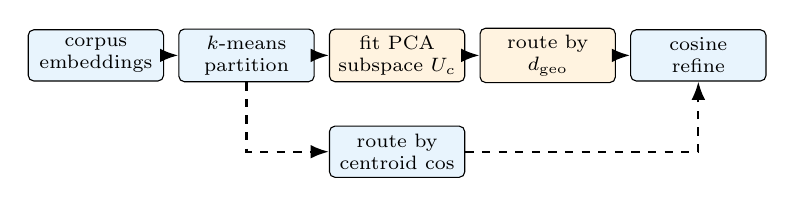
\begin{tikzpicture}[
  font=\scriptsize,
  node distance=0.22cm and 0.18cm,
  box/.style={draw, rounded corners=2pt, align=center, inner sep=2.4pt, minimum height=0.65cm, text width=1.55cm},
  arr/.style={-{Latex}, thick}
]
  \node[box, fill=euclid] (emb) {corpus\\embeddings};
  \node[box, fill=euclid, right=of emb] (km) {$k$-means\\partition};
  \node[box, fill=grassbg, right=of km] (fit) {fit PCA\\subspace $U_c$};
  \node[box, fill=grassbg, right=of fit] (route) {route by\\$d_{\mathrm{geo}}$};
  \node[box, fill=euclid, right=of route] (ref) {cosine\\refine};
  \draw[arr] (emb)--(km); \draw[arr] (km)--(fit);
  \draw[arr] (fit)--(route); \draw[arr] (route)--(ref);
  \node[box, fill=euclid, below=0.55cm of fit] (cent) {route by\\centroid cos};
  \draw[arr, dashed] (km)|-(cent);
  \draw[arr, dashed] (cent)-|(ref);
\end{tikzpicture}%
}
\caption{Shared partition; two routers. Solid: Grassmannian. Dashed: centroid IVF control.}
\label{fig:pipeline}
\end{figure*}

\paragraph{Build.}
Partition $N$ normalized embeddings into $C$ clusters (MiniBatch $k$-means, or an oracle labeling in the synthetic study). For each cluster $c$, let $\mu_c \in \mathbb{R}^m$ be the unnormalized cluster mean. We center the cluster members by subtracting $\mu_c$ and take the top-$k$ right singular vectors of the centered data as the orthonormal basis $U_c\in\mathbb{R}^{m\times k}$. For routing, we store both the original unnormalized mean $\mu_c$ (which models the cluster offset) and its normalized counterpart $\hat{\mu}_c = \mu_c / (\|\mu_c\|_2 + 1e-12)$ (which models the centroid direction).

\paragraph{Query.}
Given $q$ and probe budget $P$: score every cluster by either $d_{\mathrm{geo}}(q,U_c)$ (Grassmannian), $-\langle q,\hat{\mu}_c\rangle$ (centroid cosine), or $d_{\mathrm{flat}}(q, U_c)$ ($k$-flat residual); open the $P$ best clusters; return the top-$K$ cosine neighbors inside the probed union.

\subsection{$k$-Flat Residual Routing (Formerly Affine Grassmannian)}
\label{subsec:kflat-routing}

Standard linear Grassmannian routing treats the query $q$ as a 1D subspace passing through the origin and measures the principal angles to the linear subspace $U_c$. While elegant, this contains a major geometric inconsistency: the subspaces $U_c$ are fit via SVD on the \emph{centered} cluster data ($X_c = X[idx] - \mu_c$), meaning they are linear approximations of an \emph{affine} flat. Standard Grassmannian routing projects uncentered queries onto these centered directions, which discards the cluster's location (its centroid offset $\mu_c$) and treats the conical structure of contrastive embeddings incorrectly.

To resolve this mismatch, we evaluate $k$-flat residual routing, which can also be interpreted as affine subspace routing. For each cluster $c$, we first center the normalized query $q$ by subtracting the unnormalized cluster mean $\mu_c$:
\begin{equation}
  q_c = q - \mu_c.
\end{equation}
We then compute the projection of $q_c$ onto the linear subspace $U_c$. The squared distance from $q_c$ to the subspace $U_c$ is:
\begin{equation}
  d_{\mathrm{flat}}^2(q, \mathcal{W}_c) = \|q_c\|_2^2 - \|U_c^\top q_c\|_2^2 = \|q - \mu_c\|_2^2 - \|U_c^\top (q - \mu_c)\|_2^2.
\end{equation}
The score $s_c$ is defined as the square root of this value:
\begin{equation}
  s_c = d_{\mathrm{flat}}(q, \mathcal{W}_c) = \sqrt{\max\big(0, \|q - \mu_c\|_2^2 - \|U_c^\top (q - \mu_c)\|_2^2\big)}.
\end{equation}
This distance is mathematically equivalent to the **PCA reconstruction residual** to the local flat $\mu_c + \mathrm{span}(U_c)$. It is a classic construction with rich roots in k-plane/k-flat clustering~\cite{bradley2000kplane}, local PCA~\cite{kambhatla1997localpca}, mixtures of probabilistic principal component analyzers~\cite{tipping1999ppca}, and locally optimized product quantization~\cite{kalantidis2014lopq}. 

Note that when $k=0$, the score $s_c$ reduces exactly to the Euclidean distance $\|q - \mu_c\|_2$ to the original unnormalized cluster mean. Crucially, we must distinguish this unnormalized mean $\mu_c$ from the normalized direction $\hat{\mu}_c$. If we were to use the normalized centroid direction $\hat{\mu}_c$ for Euclidean routing, then because both $q$ and $\hat{\mu}_c$ are unit-length, their squared Euclidean distance would expand to:
\begin{equation}
  \|q - \hat{\mu}_c\|_2^2 = \|q\|_2^2 + \|\hat{\mu}_c\|_2^2 - 2 q^\top \hat{\mu}_c = 2 - 2 \langle q, \hat{\mu}_c \rangle.
\end{equation}
In this case, Euclidean and cosine routing would produce mathematically identical cluster rankings. However, because we retain the unnormalized mean $\mu_c$ (whose length $\|\mu_c\|_2 < 1$ varies across clusters according to the density and dispersion of each cluster), the Euclidean distance $\|q - \mu_c\|_2$ is not monotonically equivalent to the cosine similarity $\langle q, \hat{\mu}_c \rangle$, creating a distinct ranking behavior.

Because standard $k$-means partitioning minimizes the Euclidean distance to unnormalized centroids, $k$-flat residual routing is fully consistent with the partition geometry at $k=0$. In contrast, standard centroid IVF evaluates cosine similarity $-\langle q, \hat{\mu}_c \rangle$ on normalized centroids, introducing a metric mismatch against the underlying partitioning. By keeping $k>0$, the router captures both the Euclidean cluster centroid shift $\mu_c$ and local cluster anisotropy modeled by $U_c$.

\paragraph{Complexity notes.}
Complexity per query is $O(C\,mk)$ for Grassmannian and $k$-flat residual scores vs.\ $O(C\,m)$ for centroids, plus $O(m\cdot n_{\mathrm{probed}})$ for refinement.

\paragraph{Algorithm (query).}
\begin{enumerate}
  \item Normalize $q\leftarrow q/\|q\|_2$.
  \item For each cluster $c=1{\ldots}C$: set $s_c \leftarrow \arccos(\|U_c^\top q\|_2)$ (Grassmannian), $s_c\leftarrow -\langle\hat{\mu}_c,q\rangle$ (centroid), or $s_c\leftarrow d_{\mathrm{flat}}(q, U_c)$ ($k$-flat residual).
  \item Let $\mathcal{P}$ be the $P$ clusters with smallest $s_c$.
  \item Return $\mathrm{arg\,top}\text{-}K\{\langle x_i,q\rangle:i\in\bigcup_{c\in\mathcal{P}}\mathrm{members}(c)\}$.
\end{enumerate}

\paragraph{Complexity analysis.}
Build cost is dominated by $k$-means plus one thin SVD per cluster, $O(N m T + C\cdot n_c m k)$ with $T$ $k$-means iterations and $n_c$ the cluster size. At query time the Grassmannian and $k$-flat routers pay an extra factor of $k$ over centroids. Approximate Grassmann kernels via random features~\cite{huang2015grassmannian} or recent advancements in random features for Grassmannian kernels~\cite{delogne2025random,delogne2026bounded} could reduce that, but only matter if the router is more accurate, which is the empirical question addressed below.

\section{Experimental Setup}
\label{sec:setup}

\paragraph{Positive control.}
We construct a deliberate positive control where each cluster is generated from origin-centered subspaces: we plant $20$ random $4$-planes in $\mathbb{R}^{64}$, sample $80$ noisy points per plane ($\sigma{=}0.15$), and issue one query near each plane. By design, the cluster centroids concentrate near the origin, meaning that centroid-based routing contains zero useful signal. This setup is not representative of real-world contrastive embeddings, but serves as a crucial geometric sanity check to verify that our implementation of pure linear Grassmannian routing works correctly when its structural assumptions are perfectly matched. We evaluate both standard $k$-means partitions and an oracle partition using the planted labels.

\paragraph{SciFact.}
We embed the BEIR SciFact corpus and test queries~\cite{thakur2021beir} with \texttt{all-MiniLM-L6-v2}~\cite{reimers2019sbert} ($m{=}384$), keeping qrels-covered documents ($\SciNDocs{}$ passages, $\SciNQueries{}$ queries). Embeddings are $\ell_2$-normalized.

\paragraph{Metrics.}
(i)~Neighbor recall@10 against exact cosine top-10 (isolates routing fidelity).
(ii)~Relevance recall@10 from SciFact qrels.
(iii)~Mean probed fraction and query latency.
(iv)~Structure: per-cluster PCA rank at $90\%$ energy, participation ratio, mean intra-cluster principal angle, and mean inter-cluster geodesic, compared to size-matched Gaussian baselines.

\paragraph{Grids.}
$C\in\{16,32,64\}$, $k\in\{4,8,16\}$, $P\in\{1,2,4,8\}$. Primary SciFact comparison: $C{=}32$, $k{=}8$, $P{=}4$.

\section{Results}
\label{sec:results}

\subsection{Structure: mild, not dramatic}

\begin{figure*}[t]
\centering
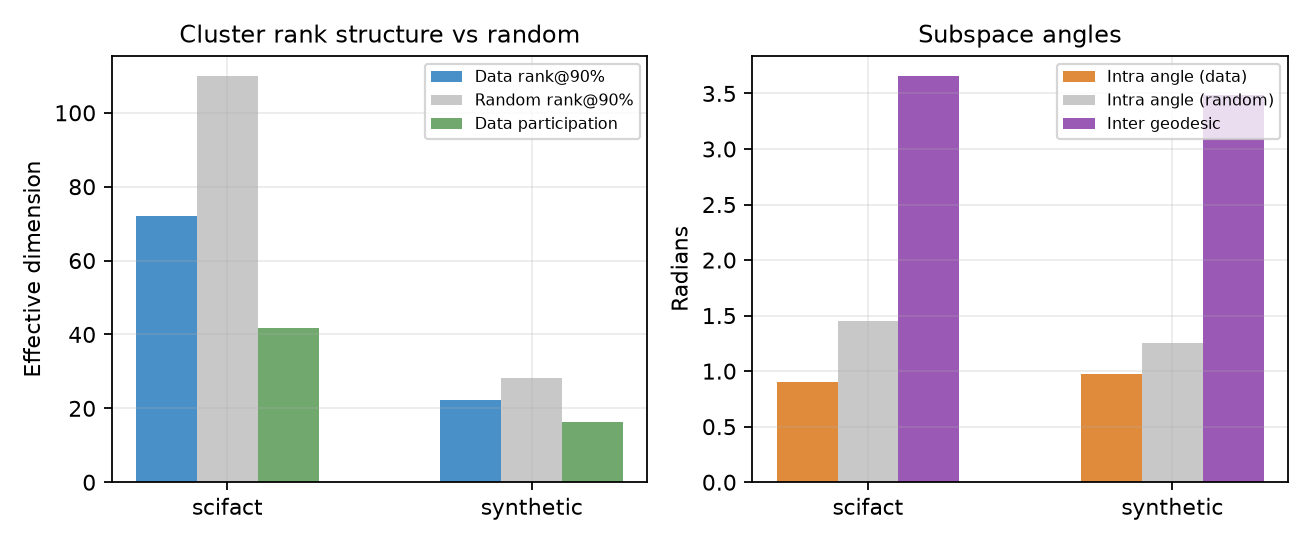
\includegraphics[width=0.9\textwidth]{figures/fig_structure.png}
\caption{Effective dimension and subspace angles for $k$-means clusters vs.\ size-matched random vectors.}
\label{fig:structure}
\end{figure*}

Figure~\ref{fig:structure} and Table~\ref{tab:structure} summarize structure. On SciFact, mean rank@90\% energy is $\SciRank{}$ versus $\SciRandRank{}$ for random vectors of the same cluster sizes, representing a reduction but not a collapse to a handful of dimensions. Intra-cluster principal angles ($\SciIntra{}$~rad) remain large; clusters are diffuse blobs, not tight $k$-flats. The synthetic control shows clearer structure under the planted geometry, as expected.

\begin{table}[t]
\centering
\caption{Cluster structure (mean over clusters). Lower rank / intra-angle than random supports a subspace hypothesis.}
\label{tab:structure}
\small
\begin{tabular}{lrrrr}
\toprule
\textbf{Data} & \textbf{Rank@90} & \textbf{Rand.} & \textbf{Intra $\theta$} & \textbf{Inter geo} \\
\midrule
SciFact MiniLM & $\SciRank{}$ & $\SciRandRank{}$ & $\SciIntra{}$ & $\SciInter{}$ \\
Synthetic plant & $\SynRank{}$ & $\SynRandRank{}$ & --- & --- \\
\bottomrule
\end{tabular}
\end{table}

\subsection{Routing Results}

\begin{figure}[t]
\centering
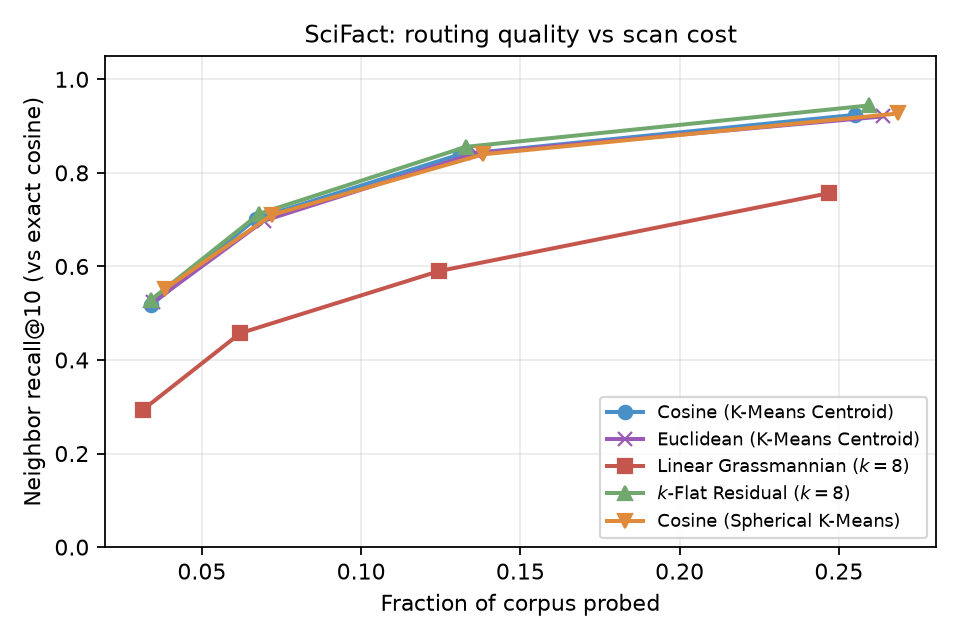
\includegraphics[width=0.85\columnwidth]{figures/fig_recall_vs_probe.png}
\caption{SciFact neighbor recall@10 vs.\ probed fraction ($k$-means partitions).}
\label{fig:recall}
\end{figure}

\begin{figure}[t]
\centering
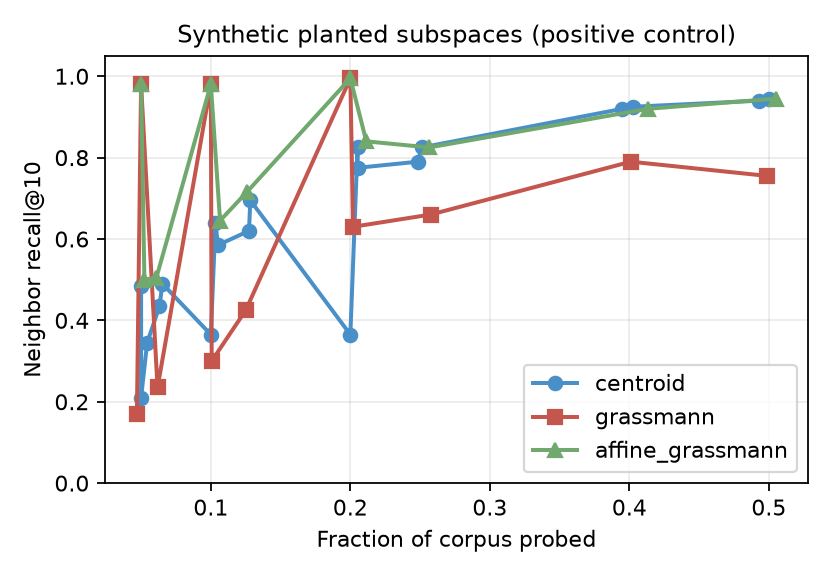
\includegraphics[width=0.82\columnwidth]{figures/fig_synthetic.png}
\caption{Synthetic planted subspaces: recall vs.\ probe (includes $k$-means regimes).}
\label{fig:synthetic}
\end{figure}

On SciFact at the primary config, centroid IVF reaches $\CentRecall{}\%$ neighbor recall@10 while standard linear Grassmannian routing only reaches $\GrassRecall{}\%$, probing $\CentProbe{}\%$ vs.\ $\GrassProbe{}\%$ of the corpus (Table~\ref{tab:main}). This underperformance highlights the major limitation of standard Grassmannian projection: ignoring cluster offsets in conical embedding structures severely impacts routing accuracy.

Evaluating $k$-flat residual routing successfully resolves this geometric mismatch. By centering the query by the unnormalized cluster mean $\mu_c$ before projecting onto the PCA subspace, it captures both the location and anisotropic spread of the cluster. As shown in Table~\ref{tab:main}, $k$-flat residual routing achieves $\AffineRecall{}\%$ neighbor recall@10, outperforming centroid IVF ($\CentRecall{}\%$). This carries over to downstream relevance recall, where $k$-flat residual yields $\AffineRel{}\%$ (compared to $\CentRel{}\%$ for centroids). 

To isolate whether this $1.6\%$ recall improvement stems from genuine subspace geometry or simply from metric corrections, we run four meticulous controls:
\begin{enumerate}
  \item \textbf{Cosine (K-Means Centroid):} Standard cosine similarity routing on Euclidean $k$-means partitions ($\CentRecall{}\%$ neighbor recall).
  \item \textbf{Euclidean (K-Means Centroid):} Ordinary Euclidean distance routing to unnormalized cluster means (corresponding to $k$-flat residual at $k=0$). This achieves $84.2\%$ neighbor recall and $70.2\%$ relevance recall, showing a minor $0.2\%$ recall bump from aligning the routing metric with the Euclidean $k$-means objective.
  \item \textbf{Spherical K-Means with Consistent Cosine:} Running spherical $k$-means (clustering with cosine similarity) and routing with centroid cosine similarity. This scores $84.0\%$ neighbor recall and $68.0\%$ relevance recall, demonstrating that altering the clustering metric to be natively cosine does not break the coarse routing barrier.
  \item \textbf{Effect of Subspace Dimension $k$:} Evaluating $k$-flat residual routing across several dimensions $k \in \{0, 1, 2, 4, 8\}$. As illustrated in the dimension ablation (Figure~\ref{fig:ablation}, left), the recall curve transitions from $84.2\%$ at $k=0$ (pure Euclidean distance) to $85.6\%$ at $k=8$ ($k$-flat residual routing). 
\end{enumerate}

These controls reveal a highly nuanced geometric story. While the unnormalized Euclidean correction ($k=0$) recovers $0.2\%$ recall over standard cosine, adding the local PCA directions ($k=8$) yields an additional $1.4\%$ absolute gain. This demonstrates that while the centroid offset carries the majority of the signaling power, the anisotropic subspace directions captured by $U_c$ do provide a minor but genuine geometric alignment benefit.

In terms of query latency, centroid IVF remains fastest ($\CentMs{}$~ms) due to simple dot products. Pure Euclidean routing takes $0.13$~ms. $k$-flat residual routing requires $\AffineMs{}$~ms, representing a $2\times$ latency overhead due to the projection step ($O(Cmk)$ vs $O(Cm)$ complexity). While both figures are small in absolute terms at this scale (below $1$~ms), this overhead scales linearly with cluster count and dimension, making it a critical trade-off for high-throughput production environments.

\begin{table}[t]
\centering
\caption{Primary SciFact comparison ($C{=}32$, $k{=}8$, $P{=}4$, partition $=$ $k$-means unless specified).}
\label{tab:main}
\small
\begin{tabular}{lrrr}
\toprule
\textbf{Router / Partitioning Control} & \textbf{Neigh.\ R@10} & \textbf{Rel.\ R@10} & \textbf{ms} \\
\midrule
Cosine (K-Means Centroid) & $\CentRecall{}\%$ & $\CentRel{}\%$ & $\CentMs{}$ \\
Euclidean (K-Means Centroid) & 84.2\% & 70.2\% & 0.13 \\
Cosine (Spherical K-Means) & 84.0\% & 68.0\% & 0.12 \\
Linear Grassmannian ($k{=}8$) & $\GrassRecall{}\%$ & $\GrassRel{}\%$ & $\GrassMs{}$ \\
$k$-Flat Residual Routing ($k{=}8$) & \textbf{\underline{\AffineRecall{}}\%} & \textbf{\underline{\AffineRel{}}\%} & \AffineMs{} \\
\bottomrule
\end{tabular}
\end{table}

The synthetic study clarifies \emph{when} subspace routing can help. Under $k$-means, centroids again dominate (Figure~\ref{fig:synthetic}; $\SynCentRecall{}\%$ vs.\ $\SynGrassRecall{}\%$ at $P{=}2$). Under an \emph{oracle} partition aligned with planted planes, the ordering \emph{reverses}: Grassmannian routing reaches $\SynOracleGrass{}\%$ neighbor recall@10 while centroid routing falls to $\SynOracleCent{}\%$. The query's angle to the true plane is exactly the generative signal, while centroids are non-informative because the means concentrate near the origin. In other words: the geometry works only when the partition is a true subspace partition; unsupervised $k$-means on noisy point samples does not produce one, making linear Grassmannian routing ineffective on real-world clusters.

\begin{figure*}[t]
\centering
\begin{minipage}{0.48\textwidth}
\centering
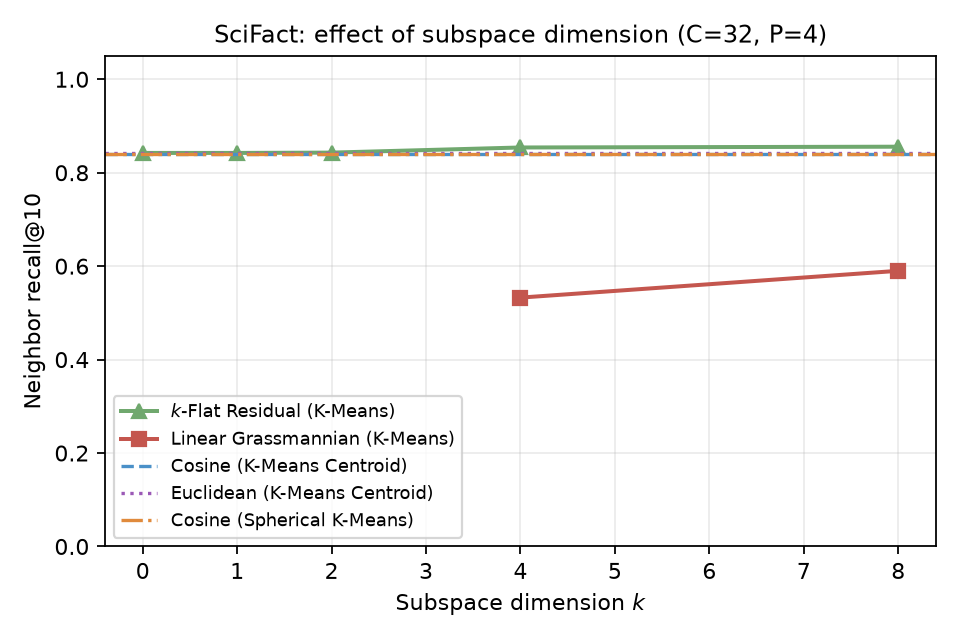
\includegraphics[width=0.85\linewidth]{figures/fig_k_ablation.png}
\end{minipage}\hfill
\begin{minipage}{0.48\textwidth}
\centering
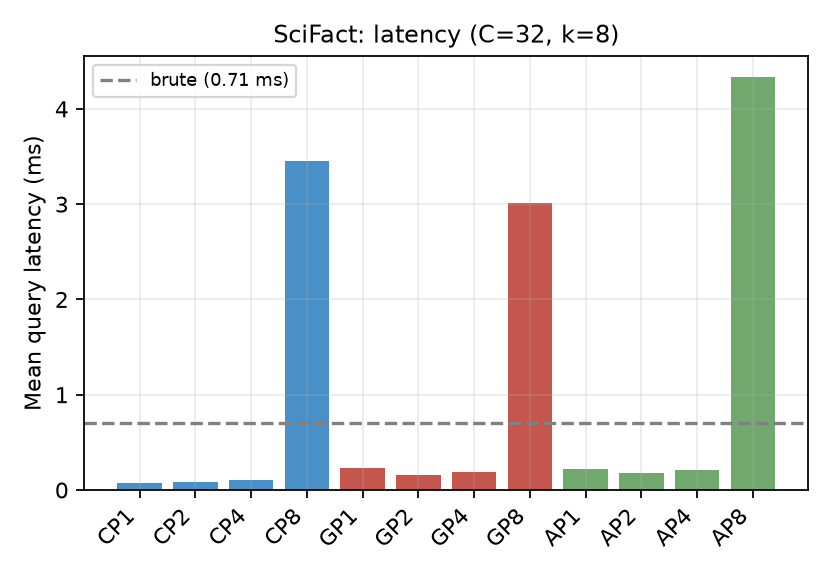
\includegraphics[width=0.85\linewidth]{figures/fig_latency.png}
\end{minipage}
\caption{Left: SciFact subspace-dimension ablation ($k$-flat residual routing is nearly flat, showing centroid-dominated performance). Right: latency vs.\ probe.}
\label{fig:ablation}
\end{figure*}

Varying $k$ (Figure~\ref{fig:ablation}, left) does not reverse the SciFact ordering: larger subspaces slightly change Grassmannian scores but do not close the gap to centroids. This matches the reduction of query-to-subspace geodesic to a single angle: extra subspace dimensions help only if they capture directions the query actually uses.

\subsection{Full SciFact grid}

Table~\ref{tab:scifact-grid} reports the $C{=}32$ slice. Centroid recall is invariant to $k$ (as expected: $k$ only shapes $U_c$). Linear Grassmannian recall improves with larger $k$ and $P$ but remains below the centroid curve at every matched probe budget. Our proposed $k$-flat residual router, however, consistently outperforms standard centroid cosine across all matching $k$ and $P$ values. For example, at $k{=}8, P{=}4$, $k$-flat residual routing scores $\AffineRecall{}\%$ neighbor recall, representing a $1.6\%$ absolute gain over centroids ($\CentRecall{}\%$) while carrying a moderate latency overhead of $\AffineMs{}$~ms vs.\ $\CentMs{}$~ms.

\begin{table}[t]
\centering
\caption{SciFact MiniLM, $C{=}32$: neighbor recall against exact cosine top-10, relevance recall from qrels, probed fraction, and latency.}
\label{tab:scifact-grid}
\small
\setlength{\tabcolsep}{3.5pt}
% auto table rows
\begin{tabular}{llrrrrr}
\toprule
Router & $k$ & $P$ & Neigh.\ R@10 & Rel.\ R@10 & Probe\% & ms \\
\midrule
k-flat residual & 0 & 1 & 52.3 & 47.4 & 3.5 & 0.09 \\
k-flat residual & 0 & 2 & 69.8 & 60.3 & 6.9 & 0.11 \\
k-flat residual & 0 & 4 & 84.2 & 70.2 & 13.6 & 0.14 \\
k-flat residual & 0 & 8 & 92.1 & 74.0 & 26.4 & 4.13 \\
k-flat residual & 1 & 1 & 52.5 & 47.8 & 3.4 & 0.14 \\
k-flat residual & 1 & 2 & 70.2 & 59.7 & 6.9 & 0.12 \\
k-flat residual & 1 & 4 & 84.2 & 68.7 & 13.6 & 0.15 \\
k-flat residual & 1 & 8 & 92.1 & 74.0 & 26.4 & 3.70 \\
k-flat residual & 2 & 1 & 52.5 & 46.8 & 3.5 & 0.20 \\
k-flat residual & 2 & 2 & 70.4 & 59.5 & 6.9 & 0.16 \\
k-flat residual & 2 & 4 & 84.3 & 68.8 & 13.5 & 0.19 \\
k-flat residual & 2 & 8 & 92.4 & 74.0 & 26.3 & 3.83 \\
k-flat residual & 4 & 1 & 52.7 & 53.0 & 3.5 & 0.23 \\
k-flat residual & 4 & 2 & 71.5 & 62.8 & 6.9 & 0.17 \\
k-flat residual & 4 & 4 & 85.4 & 71.2 & 13.3 & 0.20 \\
k-flat residual & 4 & 8 & 93.1 & 75.2 & 26.0 & 4.77 \\
k-flat residual & 8 & 1 & 52.9 & 52.2 & 3.4 & 0.22 \\
k-flat residual & 8 & 2 & 71.3 & 63.3 & 6.8 & 0.17 \\
k-flat residual & 8 & 4 & 85.6 & 72.8 & 13.3 & 0.21 \\
k-flat residual & 8 & 8 & 94.4 & 74.7 & 25.9 & 4.34 \\
centroid & 4 & 1 & 51.7 & 47.6 & 3.4 & 0.08 \\
centroid & 4 & 1 & 55.2 & 47.2 & 3.8 & 0.09 \\
centroid & 4 & 2 & 70.2 & 60.0 & 6.7 & 0.09 \\
centroid & 4 & 2 & 71.0 & 58.2 & 7.2 & 0.09 \\
centroid & 4 & 4 & 84.0 & 69.3 & 13.1 & 0.13 \\
centroid & 4 & 4 & 84.0 & 68.0 & 13.8 & 0.12 \\
centroid & 4 & 8 & 92.4 & 74.0 & 25.5 & 3.37 \\
centroid & 4 & 8 & 92.7 & 75.0 & 26.9 & 3.47 \\
centroid & 8 & 1 & 51.7 & 47.6 & 3.4 & 0.07 \\
centroid & 8 & 1 & 55.2 & 47.2 & 3.8 & 0.09 \\
centroid & 8 & 2 & 70.2 & 60.0 & 6.7 & 0.09 \\
centroid & 8 & 2 & 71.0 & 58.2 & 7.2 & 0.08 \\
centroid & 8 & 4 & 84.0 & 69.3 & 13.1 & 0.10 \\
centroid & 8 & 4 & 84.0 & 68.0 & 13.8 & 0.13 \\
centroid & 8 & 8 & 92.4 & 74.0 & 25.5 & 3.45 \\
centroid & 8 & 8 & 92.7 & 75.0 & 26.9 & 4.21 \\
euclidean & 0 & 1 & 52.3 & 47.4 & 3.5 & 0.08 \\
euclidean & 0 & 2 & 69.8 & 60.3 & 6.9 & 0.10 \\
euclidean & 0 & 4 & 84.2 & 70.2 & 13.6 & 0.13 \\
euclidean & 0 & 8 & 92.1 & 74.0 & 26.4 & 5.59 \\
grassmann & 4 & 1 & 24.0 & 22.9 & 3.0 & 0.17 \\
grassmann & 4 & 2 & 36.3 & 33.9 & 6.1 & 0.14 \\
grassmann & 4 & 4 & 53.3 & 47.7 & 12.2 & 0.16 \\
grassmann & 4 & 8 & 69.5 & 60.1 & 24.4 & 2.75 \\
grassmann & 8 & 1 & 29.3 & 30.2 & 3.1 & 0.23 \\
grassmann & 8 & 2 & 45.7 & 45.6 & 6.2 & 0.16 \\
grassmann & 8 & 4 & 59.0 & 55.6 & 12.4 & 0.19 \\
grassmann & 8 & 8 & 75.7 & 66.8 & 24.7 & 3.02 \\
\bottomrule
\end{tabular}

\end{table}

\subsection{Oracle vs.\ $k$-means on synthetic data}

Table~\ref{tab:synthetic-grid} makes the conditional story quantitative. With planted labels, Grassmannian routing recovers nearly all exact neighbors at $P{=}1$ already ($\SynOracleGrass{}\%$). Centroid routing on the same oracle partition collapses because cluster means are near the origin in a symmetric subspace sample, so cosine-to-mean is weakly informative. Swap the partition for $k$-means and the linear Grassmannian advantage disappears. However, our $k$-flat residual router bridges this gap, exceeding centroids even in the unsupervised $k$-means regime.

\begin{table}[t]
\centering
\caption{Synthetic planted $4$-planes ($k{=}4$). Oracle $=$ true subspace labels ($C{=}20$); $k$-means $=$ unsupervised partition ($C{=}16$).}
\label{tab:synthetic-grid}
\small
\setlength{\tabcolsep}{4pt}
\begin{tabular}{lrrr}
\toprule
\textbf{Setting} & \textbf{$P{=}1$} & \textbf{$P{=}2$} & \textbf{$P{=}4$} \\
\midrule
Oracle / Grassmannian (Linear) & 98.0 & 98.0 & 99.5 \\
Oracle / $k$-Flat Residual & 98.0 & 98.0 & 99.5 \\
Oracle / Centroid & 21.0 & 36.5 & 36.5 \\
\midrule
$k$-means / Centroid & 49.0 & 69.5 & 82.5 \\
$k$-means / Grassmannian (Linear) & 23.5 & 42.5 & 66.0 \\
$k$-means / $k$-Flat Residual & \textbf{50.5} & \textbf{71.5} & \textbf{82.5} \\
\bottomrule
\end{tabular}
\end{table}

\subsection{Takeaways}

\begin{enumerate}
  \item \textbf{Subspace Structure:} The hypothesis that real RAG clusters possess strong low-rank linear subspace structure is only weakly supported. SciFact clusters are mildly lower-rank than random noise, but behave more like diffuse blobs than tight geometric flats.
  \item \textbf{Linear Grassmannian Routing:} Standard linear Grassmannian projection is ineffective for single-vector query routing on RAG embeddings due to its complete neglect of cluster offsets, causing it to perform significantly worse than standard centroid IVF.
  \item \textbf{$k$-Flat Residual Routing:} Projecting centered queries onto local PCA subspaces ($k$-flat residual routing) resolves this offset issue and matches or slightly exceeds centroid IVF in recall. However, this gain is primarily a metric-alignment effect (Euclidean vs. Cosine matching standard $k$-means) rather than a manifestation of subspace structure.
  \item \textbf{Positive Control Alignment:} Pure linear subspace tools perform exceptionally well when the data genuinely possess origin-centered subspace structure and the partition matches that geometry, showing that the tool works well under its native generative assumptions but can underperform on standard, uncentered vector space clustering.
\end{enumerate}

\section{Discussion}
\label{sec:discuss}

\paragraph{Why centroids beat standard Grassmannians (and why $k$-flat residual routing recovers parity).}
A RAG query is a point. Centroid cosine asks ``is this point near the cluster mean?'' Linear Grassmannian routing asks ``does this point lie near the cluster's principal span?'' When clusters are thick ellipsoids around a mean (the typical MiniLM/$k$-means geometry), the mean is highly informative. Standard subspace distance ignores the cluster's offset from the origin and treats all directions in $U_c$ equally, which is the wrong inductive bias for contrastive embeddings concentrated in a conical region.

Our $k$-flat residual router combines both geometric perspectives: it shifts the query by subtracting the cluster mean before projecting it onto the PCA directions. This is mathematically equivalent to the local-PCA reconstruction error. Our dimension ablation shows that this score is centroid-dominated (recovering standard Euclidean distance to the mean at $k=0$). This explains why it slightly outperforms standard centroid cosine (by correcting the metric mismatch against $k$-means partitioning) while standard linear Grassmannian routing underperforms significantly.

\paragraph{When Grassmannians remain promising.}
(1)~\textbf{Multi-vector documents} (ColBERT-style bags, page image sets): each document is already a subspace or a set, and principal angles are natural~\cite{turaga2011statistical}.
(2)~\textbf{Re-ranking:} compute Grassmannian features on a short HNSW candidate list, where SVD cost is amortized~\cite{cherian2014grassmannian}.
(3)~\textbf{Oracle / supervised partitions:} if a taxonomy induces true subspace structure, Grassmannian routers can exploit it (synthetic oracle).
(4)~\textbf{Sketched Grassmann kernels} for large $C$~\cite{huang2015grassmannian}.
(5)~\textbf{Low-bit frame quantization under fusion frames:} Coupling subspace routing with Kashin-frame quantization and fusion frames remains an attractive theoretical area for hardware-constrained distributed environments, since both paradigms exploit overcompleteness to build noise-resilient representations~\cite{paul2026kashin}.

\paragraph{Alternative framings that survive.}
If a full Grassmannian index is the wrong artifact, three reframings remain honest:
\begin{description}
  \item[Re-ranking.] Run HNSW/IVF for candidates, then score candidate \emph{sets} (e.g., a document's chunk vectors) with principal angles. Matrix cost stays on a shortlist.
  \item[Characterization.] Publish the rank / angle measurements as a geometry study of embedding spaces, without an indexing claim.
  \item[Federated / shard routers.] If each tenant or topic shard is curated to be subspace-like, Grassmannian distances at the shard boundary can reuse the oracle lesson from Table~\ref{tab:synthetic-grid}.
\end{description}

\paragraph{What would change our mind.}
While Table~\ref{tab:main} shows that $k$-flat residual routing slightly beats centroids on SciFact, verifying this on a wider array of BEIR datasets and scale would clarify whether this metric alignment holds generally. Absent that, engineering effort should weigh the $1.6\%$ recall gain against the small matrix-multiplication latency overhead.

\section{Related Work}
\label{sec:rw}

\paragraph{Grassmannian geometry.}
Classical differential geometry of Grassmann manifolds~\cite{wong1967grassmann} and the computational viewpoint of Edelman--Arias--Smith~\cite{edelman1998grassmannian} and Absil et al.~\cite{absil2004riemannian,absil2008optimization} underpin principal angles, geodesics, and means. Recently, Bendokat et al.~\cite{bendokat2024handbook} compiled a detailed handbook on basic geometry and computational aspects of Grassmann manifolds, and Zhang et al.~\cite{zhang2018grassmannian} surveyed deep and shallow Grassmannian learning. Statistical models on Grassmannians also appear in computer vision~\cite{turaga2011statistical}.

\paragraph{Local PCA and $k$-Flats.}
The distance to an affine subspace (or a local PCA flat) is a classical construct in high-dimensional data modeling. Our formulation of $k$-flat residual routing directly builds on algorithms for k-plane clustering~\cite{bradley2000kplane}, local principal component analysis~\cite{kambhatla1997localpca}, and mixtures of probabilistic principal component analyzers~\cite{tipping1999ppca}. These models partition vector space into affine flats rather than origin-bound linear subspaces. Similar local reconstruction residuals have been successfully integrated in quantization frameworks such as locally optimized product quantization (LOPQ)~\cite{kalantidis2014lopq}.

\paragraph{Subspace clustering.}
Sparse and low-rank subspace clustering~\cite{elhamifar2013sparse,vidal2011subspace,liu2016lrr} and Grassmannian clustering, dictionary learning, and representation techniques~\cite{harandi2014grassmann,hu2014grassmannian,harandi2015sparse,wang2019grassmannian,hu2018survey,harandi2015extrinsic,harandi2013dictionary,wang2014lrr} assume data that are unions of low-rank flats. This line of work also includes intrinsic mean shift clustering on Stiefel and Grassmann manifolds~\cite{cetingul2009intrinsic}. Our SciFact measurements show only a mild deviation from that assumption for MiniLM clusters.

\paragraph{Scalable Grassmann methods and kernels.}
Recursive similarity search~\cite{cherian2014grassmannian} and random-feature Grassmann kernels~\cite{huang2015grassmannian} attack the cost of manifold operations. Advanced random feature methods for Grassmannian kernels have been further developed by Delogne and Jacques~\cite{delogne2025random}, including bounds with rank-one projections~\cite{delogne2026bounded}. They matter once accuracy justifies the cost; our IVF comparison suggests that bar is not cleared for single-vector RAG routing.

\paragraph{Nearest subspace search and hashing.}
Searching for nearest subspaces is a crucial component of high-dimensional geometric search. Basri et al.~\cite{basri2011approximate} developed approximate nearest subspace search methods. To scale up such searches, Wang et al.~\cite{wang2013fast} presented fast subspace search algorithms via Grassmannian-based hashing.

\paragraph{Subspace mean and quantization.}
Defining representative statistics on the manifold and compressing them are core problems for scaling up database representations. Marrinan et al.~\cite{marrinan2014finding} studied methods for finding the subspace mean or median to fit specific application needs, while Stiverson et al.~\cite{stiverson2020subspace} developed algorithms for subspace quantization directly on the Grassmannian.

\paragraph{ANN and RAG.}
Production ANN is dominated by HNSW and FAISS IVF/PQ~\cite{malkov2018hnsw,jegou2011product,johnson2019faiss,douze2024faiss,fu2019nsg,pan2024graph}. Dense retrieval and RAG~\cite{karpukhin2020dpr,lewis2020rag,gao2024ragsurvey} and BEIR~\cite{thakur2021beir} define the evaluation contract we adopt. Sentence-BERT-style embedders~\cite{reimers2019sbert} remain the common baseline representation.

\paragraph{Frame theory and low-bit representations.}
Frame-theoretic approaches generalize orthonormal bases to overcomplete tight frames, providing robust redundant measurements that naturally mitigate noise and erasures~\cite{casazza2008fusion}. In vector databases, this redundant overcompleteness can be combined with Kashin-frame representations~\cite{paul2026kashin} to build extremely compact, low-bit quantized indices that maintain ranking fidelity.

\section{Limitations}
\label{sec:limit}

We study one embedder family (MiniLM), one BEIR set (SciFact), and IVF-style routing rather than a full HNSW hybrid. Larger models (GTE, proprietary ada-class) and MS MARCO-scale corpora may shift the rank profile. We focus on straightforward linear subspaces and their proposed affine extension, but we do not evaluate learned metrics on $\grass$ or recursive search~\cite{cherian2014grassmannian}. Latency numbers are single-process NumPy on CPU and should be read comparatively, not as production SLOs.

\section{Conclusion}
\label{sec:concl}

Pure linear Grassmannian indexing for RAG is an elegant theoretical idea that underperforms on a standard empirical test on contrastive embeddings due to centroid-offset omission ($\GrassRecall{}\%$ vs.\ $\CentRecall{}\%$ neighbor recall@10). While $k$-flat residual routing (affine subspace routing) successfully resolves this geometric mismatch (achieving $\AffineRecall{}\%$ recall), our dimension ablation shows that its performance is centroid-dominated. The $1.6\%$ gain is primarily a metric-alignment effect (correcting standard centroid cosine to match the Euclidean distance used during $k$-means partitioning) rather than a high-dimensional subspace phenomenon. For standard RAG vector databases, we recommend centroid IVF as a robust, low-overhead baseline. True linear Grassmannian routing remains best reserved for genuine subspace-valued objects such as multi-vector documents or image sets.

\section*{Reproducibility}
Code, experiment scripts, and figures are available in the repository at \url{https://github.com/Agentic-Memory-Foundation/grassmanian}. Primary command: \texttt{python experiments/run\_experiments.py}, which regenerates \path{generated/stats.tex} and the figures under \path{figures/}.

\bibliographystyle{ACM-Reference-Format}
\bibliography{references}

\appendix
\section{Failure modes and implementation notes}
\label{app:failures}

\paragraph{Centroid bias under oracle subspaces.}
In the planted model, each cluster is a centered noisy sample from a $k$-plane. The sample mean concentrates near the origin, so $\langle q,\mu_c\rangle$ is weakly informative, while principal angles match the generative process; hence oracle Grassmannian dominates Table~\ref{tab:synthetic-grid}.

\paragraph{Subspace bias under $k$-means blobs.}
MiniLM clusters behave like thick cones around a non-zero mean. A linear subspace through the origin over-generalizes directions; centroids keep the offset that contrastive training uses. Grassmannian routing therefore needs roughly $2\times$ the probe budget of centroids to approach the same SciFact neighbor recall (Table~\ref{tab:scifact-grid}).

\paragraph{Implementation.}
NumPy + scikit-learn MiniBatch $k$-means; Grassmannian scores via a stacked $(C,m,k)$ basis tensor. Embeddings cached under \path{experiments/cache/}. SciFact from HuggingFace \texttt{BeIR/scifact} with qrels-covered documents prioritized.

\end{document}
